\section{Auswertung}
\label{sec:Auswertung}
\subsection{Wheatstonesche Brücke}
\label{sec:Wheat}
Mit der Wheatstoneschen Brückenschaltung sollten zwei Unbekannte Widerstände ermittelt werden.
In der folgenden Tabelle werden die Messwerte $R_2$ und $\frac{R_3}{R_4}$ der Messreihe aufgelistet. Zudem ist, der mit Hilfe von Gleichung $\ref{eqn:wheat}$, berechnete 
Wert für $R_\text{x}$ eingetragen. Der Fehler lässt sich mit Hilfe der Gaußschen Fehlerfortpflanzung
\\
\begin{equation}
  \label{eqn:fehR}
  \symup{\Delta}R_x=\sqrt{\left(\frac{R_3}{R_4}\right)^2 \cdot \left(\symup{\Delta}R_2\right)^2 + R_2^2 \cdot \left(\symup{\Delta}\frac{R_3}{R_4}\right)^2}
\end{equation}
\\
berechnen. Die Fehler sind gegeben durch $\symup{\Delta}R_2$ = $\pm 0.002 \cdot R_2$
und $\symup{\Delta}\frac{R_3}{R_4}$ = $\pm 0.005 \cdot \frac{R_3}{R_4}$.
%
%
\\
\begin{table}
  \centering
  \caption{Messwerte und berechnete Werte für Widerstand $R_\text{x}$ (Wert 10)}
  \label{tab:Wheat}
  \sisetup{table-format = 4}
  \begin{tabular}{
    c
    S @{${}\pm{}$} S[table-format=1.2]
    S[table-format=1.2] @{${}\pm{}$} S[table-format=1.1]
    S[table-format = 3.2] @{${}\pm{}$} S[table-format=1.2]}
     \toprule
     {Wert 10}  &
     \multicolumn{2}{c}{$R_2 \mathbin{/} \si{\ohm}$}       &
     \multicolumn{2}{c}{$\frac{R_3}{R_4}$}       & 
     \multicolumn{2}{c} {$R_\text{x}  \mathbin{/} \si{\ohm}$}\\
     \cmidrule(lr){2-3} \cmidrule(lr){4-5} \cmidrule(lr){6-7}
     \midrule
     Messung 1 & 332  & 0.66 & 0.72 & 0.0 & 240.41 & 1.3\\
     Messung 2 & 664  & 1.33 & 0.36 & 0.0 & 238.17 & 1.28\\
     Messung 3 & 1000 & 2    & 0.24 & 0.0 & 239.93 & 1.29\\
      \bottomrule
  \end{tabular}
\end{table}%
\\
Der Mittelwert von $R_\text{x}$ lässt sich berechnen mit 
\\
\begin{equation}
  \label{eqn:mit}
  \bar{R_\text{x}}=\sum_{i=1}^3 \frac{1}{3}R_{x_i}\, .
\end{equation}
Daraus folgt für den Mittelwert des Widerstands Wert 10, $R_\text{x}= \SI{239.5\pm0.7}{\ohm}$.
Äquivalent dazu, wurden auch die Werte von dem anderen unbekannten Widerstand ermittelt und eingetragen.
%
\\
\begin{table}
  \centering
  \caption{Messwerte und berechnete Werte für Widerstand $R_\text{x}$ (Wert 11)}
  \label{tab:Wheatr}
  \sisetup{table-format = 4}
  \begin{tabular}{
    c
    S @{${}\pm{}$} S[table-format=1.2]
    S[table-format=1.2] @{${}\pm{}$} S[table-format=1.2]
    S[table-format = 3.2] @{${}\pm{}$} S[table-format=1.2]}
     \toprule
     {Wert 11}  &
     \multicolumn{2}{c}{$R_2 \mathbin{/} \si{\ohm}$}       &
     \multicolumn{2}{c}{$\frac{R_3}{R_4}$}       & 
     \multicolumn{2}{c} {$R_\text{x}  \mathbin{/} \si{\ohm}$}\\
     \cmidrule(lr){2-3} \cmidrule(lr){4-5} \cmidrule(lr){6-7}
     \midrule
     Messung 1 & 332  & 0.66  & 1.48 & 0.01 & 491.82 & 2.65\\
     Messung 2 & 664  & 1.33  & 0.74 & 0.0 & 488.78 & 2.63\\
     Messung 3 & 1000 & 2     & 0.49 & 0.0 & 492.54 & 2.65\\
      \bottomrule
  \end{tabular}
\end{table}
\\
Mit der Formel für den Mittelwert \ref{eqn:mit} folgt für Wert 11, $R_\text{x}=\SI{491\pm1.5}{\ohm}$
\newpage%
%
%
%
\subsection{Kapazitätsmessbrücke}
In der Messung um den realen Kondensator, ist dieser durch einen ohmschen Widerstand und eine widerstandslose Kapazität ersetzt worden.
Zum berechnen der Werte wurde die Gleichung $\ref{eqn:capmes}$ genutzt.
Alle Messwerte, berechneten Kapazitäten und Widerstände für den Wert 8 sind in der Tabelle \ref{tab:kapa} aufgeführt.
Dabei wurden die Fehler des Widerstands mit der Formel \ref{eqn:fehR} und
die der Kapazität mit
\\ 
\begin{equation}
  \symup{\Delta}C_x=\sqrt{\left(\frac{R4}{R3}\right)^2 \cdot \left(\symup{\Delta}C_2\right)^2
  +\left(-C_2\frac{R4}{R3}\right)^2 \cdot \left(\symup{\Delta}\frac{R4}{R3}\right)^2}
\end{equation}
\\
berechnet. Wobei $\symup{\Delta}R_2=\pm0.03 \cdot R_2$ der Fehler von dem variablen Widerstand ist und $\symup{\Delta}C_2=\pm0.002 \cdot C_2$ der Fehler 
der Kapazität. Die Abweichung von $\frac{R_3}{R_4}$ ist die selbe wie in Abschnitt \ref{sec:Wheat}.
\begin{table}
  \centering
  \caption{Messwerte und berechnete Werte für realen Kondensator, 
  $R_\text{x}$ und $C_\text{x}$ (Wert 8)}
  \label{tab:kapa}
  \sisetup{table-format = 3}
  \begin{tabular}{
    c
    S @{${}\pm{}$} S[table-format=2.2]
    S[table-format=1.2] @{${}\pm{}$} S[table-format=1.2]
    S @{${}\pm{}$} S[table-format=1.2]
    S[table-format=3.2] @{${}\pm{}$} S[table-format=2.2]
    S[table-format = 3.2] @{${}\pm{}$} S[table-format=1.2]}
     \toprule
     {Wert 8}  &
     \multicolumn{2}{c}{$R_2 \mathbin{/} \si{\ohm}$}       &
     \multicolumn{2}{c}{$\frac{R_3}{R_4}$}                 & 
     \multicolumn{2}{c}{$C_2 \mathbin{/} \si{\nano\farad}$} &
     \multicolumn{2}{c}{$R_\text{x} \mathbin{/} \si{\ohm}$}&
     \multicolumn{2}{c} {$C_\text{x}  \mathbin{/} \si{\nano\farad}$}\\
     \cmidrule(lr){2-3} \cmidrule(lr){4-5} \cmidrule(lr){6-7}
     \midrule 
     Messung 1 & 371  & 11.13  & 1.54 & 0.01 & 450 & 0.9  & 570.62& 17.35 & 292.57 & 1.58\\
     Messung 2 & 418  & 12.54  & 1.37 & 0.01 & 399 & 0.79 & 572.52& 17.41 & 291.31 & 1.57\\
     Messung 3 & 278  & 8.34   & 2.06 & 0.01 & 597 & 1.19 & 572.15& 17.4  & 290.07 & 1.56\\
      \bottomrule
  \end{tabular}
\end{table}
\\
Der Mittelwert für $R_\text{x}$ und $C_\text{x}$ wird ermittelt mit Gleichung \ref{eqn:mit} und mit \\
\begin{equation}
  \label{eqn:mit2}
  \bar{C_\text{x}}=\sum_{i=1}^3 \frac{1}{3}C_{x_i}\, .
\end{equation}
Somit bekommt man $C_\text{x}=\SI{291.3 \pm 0.9}{\nano\farad}$ und $R_\text{x}=\SI{572 \pm 10}{\ohm}$ für den Kondensator mit Wert 8.
%
\\
Äquivalent dazu wurden für den zweiten unbekannten Kondensator die Werte berechnet und in Tabelle \ref{tab:kapar} eingetragen.
\begin{table}
  \centering
  \caption{Messwerte und berechnete Werte für realen Kondensator,
   $R_\text{x}$ und $C_\text{x}$ (Wert 9)}
   \label{tab:kapar}
  \sisetup{table-format = 3}
  \begin{tabular}{
    c
    S @{${}\pm{}$} S[table-format=2.2]
    S[table-format=1.2] @{${}\pm{}$} S[table-format=1.2]
    S @{${}\pm{}$} S[table-format=1.2]
    S[table-format=3.2] @{${}\pm{}$} S[table-format=2.2]
    S[table-format = 3.2] @{${}\pm{}$} S[table-format=1.2]}
     \toprule
     {Wert 9}  &
     \multicolumn{2}{c}{$R_2 \mathbin{/} \si{\ohm}$}       &
     \multicolumn{2}{c}{$\frac{R_3}{R_4}$}                 & 
     \multicolumn{2}{c}{$C_2 \mathbin{/} \si{\nano\farad}$} &
     \multicolumn{2}{c}{$R_\text{x} \mathbin{/} \si{\ohm}$}&
     \multicolumn{2}{c} {$C_\text{x}  \mathbin{/} \si{\nano\farad}$}\\
     \cmidrule(lr){2-3} \cmidrule(lr){4-5} \cmidrule(lr){6-7}
     \midrule 
     Messung 1 & 466  & 13.98  & 1.04 & 0.01 & 450 & 0.9   & 486.97 & 14.81 & 430.63 & 2.32\\
     Messung 2 & 524  & 15.72  & 0.93 & 0.00 & 399 & 0.79  & 485.63 & 14.77 & 430.52 & 2.32\\
     Messung 3 & 352  & 10.56  & 1.39 & 0.01 & 597 & 1.19  & 488.1  & 14.84 & 430.54 & 2.32\\
      \bottomrule
  \end{tabular}
\end{table}
\\
Entsprechend der Rechnung für Wert 8, werden die Mittelwerte für Wert 9 errechnet.
Es resultiert für die Kapazität $C_\text{x}=\SI{430.6 \pm 1.3}{\nano\farad}$ und
 für den Widerstand des Kondensators $R_\text{x}=\SI{487 \pm 9}{\ohm}$ .

 \newpage
  \subsection{Induktivitätsmessbrücke}
  Bei der Induktivitätsmessbrücke wurde die reale Induktivität ersetzt durch einen ohmschen Widerstand und eine widerstandslose Induktivität.
  Zum berechnen der Werte wurde Gleichung $\ref{eqn:inducmes}$ benutzt. Die Messwerte, so wie alle errechneten Widerstände und Induktivitäten sind in der Tabelle
  \ref{tab:indu} eingetragen. Die Fehlerrechnung erfolgte mit Hilfe der Gaußschen Fehlerfortpflanzung. 
  Die Standardabweichung von $R_\text{x}$ lässt sich berechnen mit \ref{eqn:fehR}. Die Standardabweichung der Induktivität wird berechnet mit
  \begin{equation*}
    \symup{\Delta}L_x=\sqrt{\left(\frac{R_3}{R_4}\right)^2 \cdot \left(\symup{\Delta}L_2\right)^2 + L_2^2 \cdot \left(\symup{\Delta}\frac{R_3}{R_4}\right)^2}\, .
  \end{equation*}
  Für die Fehlerrechnung wurden die Fehler $\symup{\Delta}R_2=\pm0.03 \cdot R_2$ und $\symup{\Delta}L_2=\pm0.002 \cdot L_2$ angenommen. 
  $\symup{\Delta}\frac{R_3}{R_4}$ wird aus \ref{sec:Wheat} übernommen.
  \begin{table}
    \centering
    \caption{Messwerte und berechnete Werte für reale Induktivität,
     $R_\text{x}$ und $L_\text{x}$ (Wert 10)}
     \label{tab:indu}
    \sisetup{table-format = 2}
    \begin{tabular}{
      c
      S @{${}\pm{}$} S[table-format=1.2]
      S[table-format=1.2] @{${}\pm{}$} S[table-format=1.2]
      S[table-format=2.1] @{${}\pm{}$} S[table-format=1.2]
      S[table-format=3.2] @{${}\pm{}$} S[table-format=2.2]
      S[table-format = 3.2] @{${}\pm{}$} S[table-format=1.2]}
       \toprule
       {Wert 10}  &
       \multicolumn{2}{c}{$R_2 \mathbin{/} \si{\ohm}$}       &
       \multicolumn{2}{c}{$\frac{R_3}{R_4}$}                 & 
       \multicolumn{2}{c}{$L_2 \mathbin{/} \si{\milli\henry}$} &
       \multicolumn{2}{c}{$R_\text{x} \mathbin{/} \si{\ohm}$}&
       \multicolumn{2}{c} {$L_\text{x}  \mathbin{/} \si{\milli\henry}$}\\
       \cmidrule(lr){2-3} \cmidrule(lr){4-5} \cmidrule(lr){6-7}
       \midrule 
       Messung 1 & 45  & 1.35  & 9.75 & 0.05 & 14.6 & 0.03  & 438.87 & 13.35 & 142.39 & 0.77\\
       Messung 2 & 57  & 1.71  & 7.0  & 0.04 & 20.1 & 0.04  & 399    & 12.14 & 140.7  & 0.76\\
       Messung 3 & 85  & 2.55  & 5.13 & 0.03 & 27.5 & 0.06  & 436.47 & 13.27 & 141.21 & 0.76\\
        \bottomrule
    \end{tabular}
  \end{table}
  \\
  Aus den Werten von $R_\text{x}$ und $L_\text{x}$, lassen sich die Mittelwerte berechnen.
  Es ergibt sich für die Mittelwerte von Wert 10, $R_x=\SI{425\pm7}{\ohm}$ und $L_x=\SI{141.4\pm0.4}{\milli\henry}$.\\
  Für die zweite Induktivität ist die Berechnung äquivalent.
  \\
\begin{table}
  \centering
  \caption{Messwerte und berechnete Werte für reale Induktivität,
   $R_\text{x}$ und $L_\text{x}$ (Wert 18)}
   \label{tab:indul}
  \sisetup{table-format = 2}
  \begin{tabular}{
    c
    S @{${}\pm{}$} S[table-format=1.2]
    S[table-format=1.2] @{${}\pm{}$} S[table-format=1.2]
    S[table-format=2.1] @{${}\pm{}$} S[table-format=1.2]
    S[table-format=3.2] @{${}\pm{}$} S[table-format=2.2]
    S[table-format = 3.2] @{${}\pm{}$} S[table-format=1.2]}
     \toprule
     {Wert 18}  &
     \multicolumn{2}{c}{$R_2 \mathbin{/} \si{\ohm}$}       &
     \multicolumn{2}{c}{$\frac{R_3}{R_4}$}                 & 
     \multicolumn{2}{c}{$L_2 \mathbin{/} \si{\milli\henry}$} &
     \multicolumn{2}{c}{$R_\text{x} \mathbin{/} \si{\ohm}$}&
     \multicolumn{2}{c} {$L_\text{x}  \mathbin{/} \si{\milli\henry}$}\\
     \cmidrule(lr){2-3} \cmidrule(lr){4-5} \cmidrule(lr){6-7}
     \midrule 
     Messung 1 & 108  & 3.24  & 3.44 & 0.02 & 14.6 & 0.03 & 372    & 11.31 & 50.29 & 0.27\\
     Messung 2 & 143  & 4.29  & 2.51 & 0.01 & 20.1 & 0.04 & 358.75 & 10.91 & 50.43 & 0.27\\
     Messung 3 & 197  & 5.91  & 1.84 & 0.01 & 27.5 & 0.06 & 362.66 & 11.03 & 50.63 & 0.27\\
      \bottomrule
  \end{tabular}
\end{table}
\\
Es folgen die Mittelwerte für Wert 18: $R_x=\SI{364\pm6}{\ohm}$ und $L_x=\SI{50.4\pm0.16}{\milli\henry}$.
\newpage
\subsection{Maxwell-Brücke}
Für die Maxwell-Brücke wurde ein konstanter Widerstand $C_4 = \SI{399}{\nano\farad}$ verwendet. Zur Berechnung des Widerstands und der Induktivität
wurden die Gleichungen $\ref{eqn:wheat}$ und $\ref{eqn:inducmesmaxwell}$ genutzt. Die Werte wurden in die Tabelle \ref{tab:Wert10m} übertragen.\\ Es wurden die Fehler $\symup{\Delta}R_3=\pm 0.03\cdot R_3$ 
und $\symup{\Delta}R_4=\pm 0.03\cdot R_4$ verwendet. Außerdem beträgt der Fehler von $C_4$ und $R_2$ $0.2$ Prozent.
Die Fehlerrechnung für $R_\text{x}$ erfolgt über Gleichung \ref{eqn:fehR}, während der Fehler von $L_\text{x}$ mit
\begin{equation}
  \label{eqn:fehl}
  \symup{\Delta}L_x=\sqrt{\left(R_3 C_4\right)^2 \cdot \left(\symup{\Delta}R_2\right)^2 + 
  \left(R_2 C_4\right)^2 \cdot \left(\symup{\Delta}R_3\right)^2 + \left(R_2 R_3\right)^2 \cdot \left(\symup{\Delta}C_4\right)^2}
\end{equation}
berechnet wird.
\begin{table}
  \centering
  \caption{Messwerte und berechnete Werte für reale Induktivität mit Hilfe der Maxwell-Brücke,
   $R_\text{x}$ und $L_\text{x}$ (Wert 10)}
   \label{tab:Wert10m}
  \sisetup{table-format = 4}
  \begin{tabular}{
    c
    S @{${}\pm{}$} S[table-format=1.2]
    S[table-format=4] @{${}\pm{}$} S[table-format=2.2]
    S[table-format=3] @{${}\pm{}$} S[table-format=2.2]
    S[table-format=3.2] @{${}\pm{}$} S[table-format=2.2]
    S[table-format = 3.2] @{${}\pm{}$} S[table-format=1.2]}
     \toprule
     {Wert 10}  &
     \multicolumn{2}{c}{$R_2 \mathbin{/} \si{\ohm}$}       &
     \multicolumn{2}{c}{$R_3 \mathbin{/} \si{\ohm}$}                 & 
     \multicolumn{2}{c}{$R_4 \mathbin{/} \si{\ohm}$} &
     \multicolumn{2}{c}{$R_\text{x} \mathbin{/} \si{\ohm}$}&
     \multicolumn{2}{c} {$L_\text{x}  \mathbin{/} \si{\milli\henry}$}\\
     \cmidrule(lr){2-3} \cmidrule(lr){4-5} \cmidrule(lr){6-7}
     \midrule 
     Messung 1 & 1000 & 2     & 347 & 10.41 & 829 & 24.87 & 418.58& 17.78 & 138.45 & 4.17\\
     Messung 2 & 664  & 1.33  & 523 & 15.69 & 829 & 24.87 & 418.9 & 17.79 & 138.56 & 4.18\\
     Messung 3 & 332  & 0.66  & 1036& 31.08 & 829 & 24.87 & 414.9 & 17.62 & 137.24 & 4.14\\
      \bottomrule
  \end{tabular}
\end{table}
\\
Für die Mittelwerte von Wert 10 ergibt sich $R_\text{x}=\SI{417\pm10}{\ohm}$ 
und $L_\text{x}=\SI{138.1\pm 2.4}{\milli\farad}$.
\\
Die Berechnung für Wert 18 ist äquivalent.
\\
\begin{table}
  \centering
  \label{tab:Wert18m}
  \caption{Messwerte und berechnete Werte für reale Induktivität mit Hilfe der Maxwell-Brücke,
   $R_\text{x}$ und $L_\text{x}$ (Wert 18)}
  \sisetup{table-format = 4}
  \begin{tabular}{
    c
    S @{${}\pm{}$} S[table-format=1.2]
    S[table-format=4] @{${}\pm{}$} S[table-format=2.2]
    S[table-format=3] @{${}\pm{}$} S[table-format=2.2]
    S[table-format=3.2] @{${}\pm{}$} S[table-format=2.2]
    S[table-format = 3.2] @{${}\pm{}$} S[table-format=1.2]}
     \toprule
     {Wert 18}  &
     \multicolumn{2}{c}{$R_2 \mathbin{/} \si{\ohm}$}       &
     \multicolumn{2}{c}{$R_3 \mathbin{/} \si{\ohm}$}                 & 
     \multicolumn{2}{c}{$R_4 \mathbin{/} \si{\ohm}$} &
     \multicolumn{2}{c}{$R_\text{x} \mathbin{/} \si{\ohm}$}&
     \multicolumn{2}{c} {$L_\text{x}  \mathbin{/} \si{\milli\henry}$}\\
     \cmidrule(lr){2-3} \cmidrule(lr){4-5} \cmidrule(lr){6-7}
     \midrule 
     Messung 1 & 1000 & 2     & 128 & 3.84  & 347 & 10.41 & 368.88 & 15.67 & 51.07 & 1.54\\
     Messung 2 & 664  & 1.33  & 193 & 5.79  & 349 & 10.47 & 367.2  & 15.6  & 51.13 & 1.54\\
     Messung 3 & 332  & 0.66  & 382 & 11.46 & 348 & 10.44 & 364.44 & 15.48 & 50.60 & 1.52\\
      \bottomrule
  \end{tabular}
\end{table}
\\
Es ergeben sich die Mittelwerte von Wert 18: $R_\text{x}=\SI{367\pm9}{\ohm}$
 und $L_\text{x}=\SI{50.9\pm 0.9}{\milli\farad}$.
 \\
 \newpage
 \subsection{Wien-Robinson-Brücke}
 Um den Graphen zu plotten benötigt es zuerst die Frequenz $v_0$, welche in dem Versuch $v_0=\SI{162.56}{\hertz}$ beträgt.
 Beim vergleichen mit dem berrechneten Wert, $w_0= \SI{2272}{\hertz}$ ermittelt mit Hilfe der Formel $\ref{eqn:omega0}$, fällt auf, dass dieser
 sehr stark von dem beobachteten Wert abweicht.
 \begin{figure}
  \caption{Plot zu einem Frequenzfilter}
  \centering
  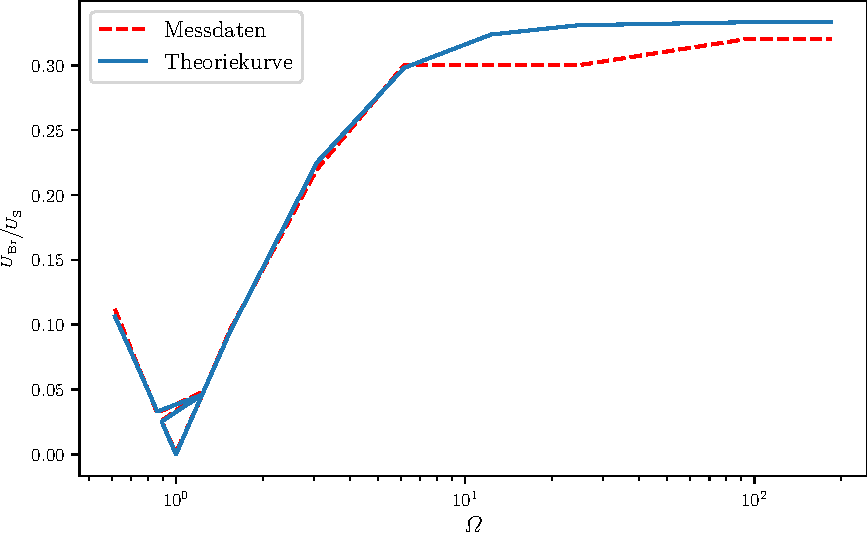
\includegraphics[width = \textwidth]{build/plot.pdf}
\end{figure}
Der Graph $\frac{U_\text{Br}}{U_S}$ ist durch die Messwerte gegeben, während der Graph $f(\Omega)$ durch die Gleichung \ref{eqn:fOmega} bestimmt wurde. 
Bei Betrachtung der Graphen fällt auf, dass die Graphen um den Punkt $\Omega=1$ sehr gut übereinstimmen.
Ab Werten mit $\Omega>10$ stimmen die Graphen nicht mehr überein. Der Graph $f(\Omega)$ stoppt früher sein Wachstum und endet so etwas tiefer, als der Graph der Messwerte.
\newpage 
\subsection{Klirrfaktor-Messung}
Zur bestimmung des Klirrfaktors wird die Summe der Oberwellen (größer als 1) auf die zweite Oberwelle beschränkt.
Mit $f(2)\approx 0.149$ und $U_\text{Br}(2v_0)=\SI{0.8}{\volt}$ folgt für die Spannung der zweiten Oberwelle $U_2=\SI{5.37}{\volt}$.
Hinzu kommt der Wert $U_1=\SI{0.009}{\volt}$, welcher für die erste Oberwelle gemessen wurde.
Dann lässt sich, mit der Formel $\ref{eqn:klirreasy}$ der Klirrfaktor, $k=596.57$ berechnen.
